\section{1. Descripción técnica-conceptual del proyecto a realizar}
\label{sec:descripcion}

Para productos de ámbitos espaciales, como lo son los satélites, muchas veces es difícil, y en ocasiones imposible, generar escenarios realistas para pruebas de los elementos que los componen. Ya sea por no poder generar las mismas condiciones ambientales, o porque la naturaleza de la maniobra que se busca probar implicaría un daño a los equipos bajo revisión.

En este contexto, es común replicar los elementos de interés de manera programada, cumpliendo con cierto grado de representación. De manera tal que se comporten de la manera más similar posible a su contraparte física. Estos elementos, íntegramente desarrollados en software, se los llaman emulados o simulados. Uno de los componentes que se suele tener mayor interés en simular es el procesador de la computadora a bordo.

El término Computadora a Bordo (OBC, por las siglas en inglés de On Board Computer) suele referirse a la unidad en la que se ejecuta el Software A Bordo (OBSW, por sus siglas en inglés de On Board Software) y su rol principal es el control de los subsistemas del satélite. Esto incluye recolectar información de diferentes subsistemas, analizarla y tomar las decisiones y acciones apropiadas cuando sea requerido.

El foco principal de este trabajo es el microprocesador contenido en la OBC. Cabe destacar, que hoy en día existen emuladores tanto de código abierto como privativos para distintos microprocesadores. Un ejemplo claro de emulador de código abierto es Qemu, que abarca un amplio abanico de microprocesadores, entre ellos, algunos utilizables en el ámbito espacial.

En el contexto de los emuladores, cada uno aborda el problema en cuestión, pero conlleva sus propias desventajas. Por ejemplo, en el caso de emuladores como Qemu, diseñados para ser genéricos, pueden requerir un esfuerzo adicional para adaptarlos a un procesador específico, como es el GR712RC. Esto se debe a que la flexibilidad genérica puede implicar una pérdida de rendimiento o la necesidad de familiarizarse con su API.

Por otro lado, los emuladores comerciales suelen estar optimizados para procesadores específicos, lo que puede brindar un excelente rendimiento en esas circunstancias particulares. Sin embargo, estos emuladores pueden ser limitados en cuanto a su capacidad de personalización, instrumentación y capacidad de integración, lo que puede dificultar su adaptación a necesidades específicas o la depuración de software en entornos no nominales.

Bajo estas premisas se plantea crear un emulador de microprocesador Leon3 para desarrollo de software satelital y simuladores. En la Figura \ref{fig:Components} se deja en evidencia un diagráma de bloques del hardware que se busca replicar. Al ser un desarrollo a medida, se tendrá la ventaja de la no-diversificación del procesador, es decir, estará únicamente orientado a un solo microprocesador. Esperando una ganancia en performance comparado con su contraparte de código abierto. Al mismo tiempo, se tendrá un conocimiento extenso del alcance y limitaciones de las capacidades del software en cuestión. Haciendo, de esta manera, más simple la integración y depuración en su uso.

\begin{figure}[htpb]
\centering
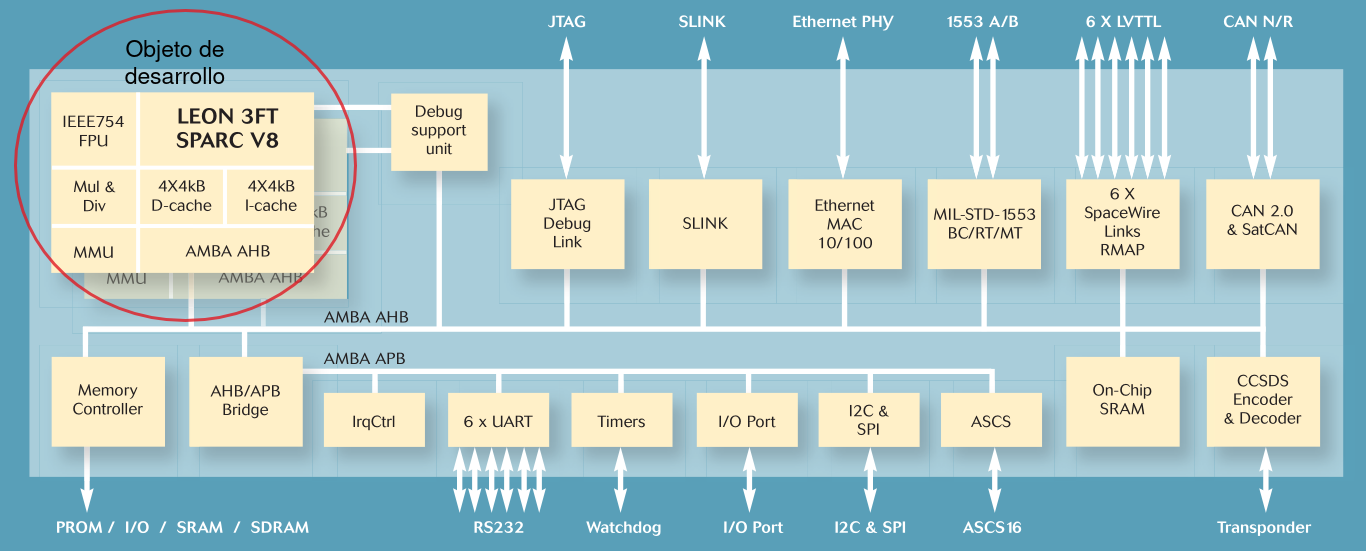
\includegraphics[width=1\textwidth]{./assets/Components.png}
\caption{Diagrama en bloques del sistema}
\label{fig:Components}
\end{figure}

\vspace{25px}

\newpage

Para lograr el objetivo descrito, se ha decidido utilizar el framework LLVM. Este se empleará para generar el conjunto de instrucciones admitido por el microprocesador Leon3. La elección de LLVM se fundamenta en varios factores clave que hacen de esta plataforma una opción sólida y versátil. Tales como que cuenta con una comunidad de desarrollo activa y comprometida, lo que garantiza un soporte continuo y actualizaciones regulares que son esenciales para mantener la robustez y eficiencia del sistema. También, al poseer soporte nativo con Leon3, es una fuente de análisis y guía en los casos donde los manuales no sean lo suficientemente claros.

Por último, es importante subrayar que el presente trabajo no se iniciará desde cero, sino que se aprovechará una base de código preexistente gentilmente proporcionada por el director de tesis. Esta base no solo servirá como una hoja de guía para el proceso de desarrollo, sino que también desempeñará un papel clave en la aceleración de todo el proyecto.
